\chapter{Evaluation}
\label{chap:evaluation}

The task of the evaluation is to check to what extent the objectives of the
work were reached. Section~7.1 describes the experimental setup,
Sections~7.2 and~7.3 report the results on SplitMNIST and PermutedMNIST,
Section~7.4 analyses why the first MoE architecture fails on PermutedMNIST,
Section~7.5 evaluates the resulting architecture variant, Section~7.6
analyses the behaviour of the router, and Section~7.7 discusses the
findings.

\section{Experimental Setup}
\label{sec:setup}

Both benchmarks consist of five tasks and were constructed exactly as
described in Section~5.3. SplitMNIST is evaluated in the task incremental
multi head protocol, PermutedMNIST in the domain incremental protocol with
one shared ten class head. All approaches see the identical task sequence,
the identical data order and the identical pixel permutations, because all
random choices are derived from controlled seeds.

Four approaches are compared in the main experiment: the naive MLP, the MLP
with EWC ($\lambda = 500$), the wide naive MLP and the MoE model with
hidden level routing (eight experts, top $2$, load balancing coefficient
$\alpha = 0.01$). Every model is trained with the Adam optimiser, learning
rate $10^{-3}$, for five epochs per task with a mini batch size of $256$.
All experiments are repeated with the three seeds $\{0, 1, 2\}$, and all
reported numbers are means over these seeds with the standard deviation.

After every training stage, the model is evaluated on the test sets of all
tasks seen so far, which gives the accuracy matrix $R$. From the final
matrix, the average accuracy $A$, the average forgetting $F$ and the
backward transfer BWT are derived, as defined in Section~2.4.
Figure~7.1 summarises the two most important metrics for all approaches
and both benchmarks.

\begin{figure}[H]
  \centering
  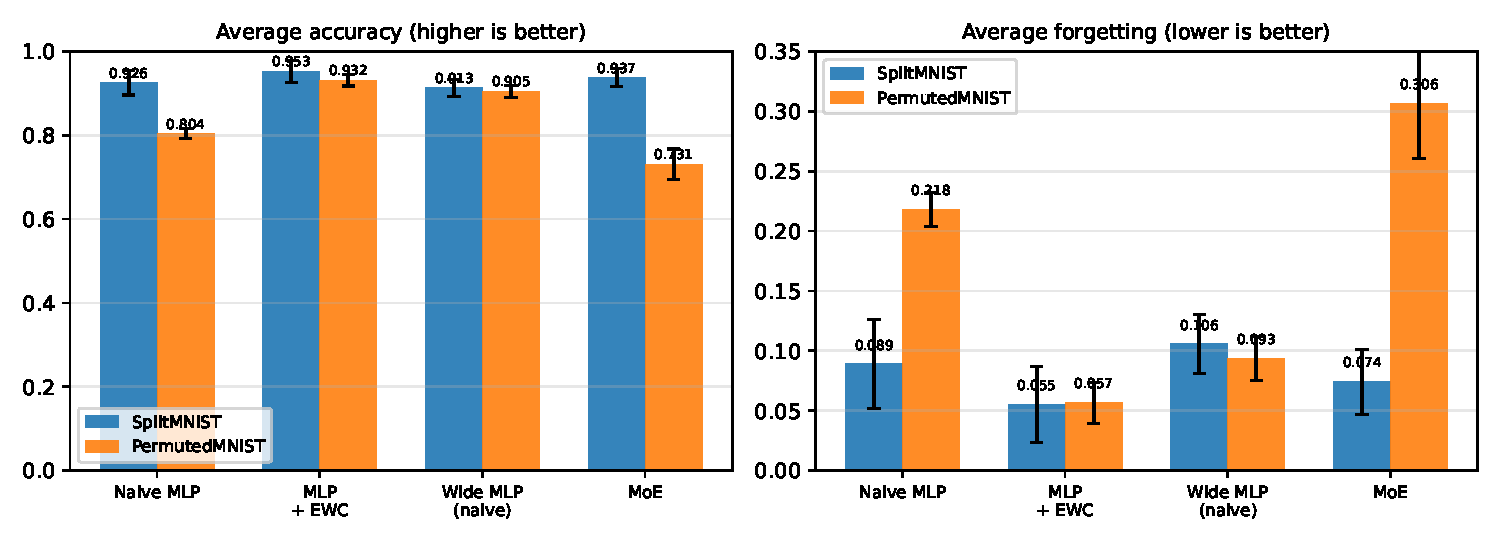
\includegraphics[width=\textwidth]{figures/metrics_summary.pdf}
  \caption{Average accuracy (left) and average forgetting (right) of all
  compared approaches on both benchmarks (mean over three seeds, error bars
  show the standard deviation).}
  \label{fig:metrics_summary}
\end{figure}

The computational cost of the approaches differs noticeably, which is part
of the practical trade off. Table~\ref{tab:runtimes} lists the mean runtime of one
complete continual run (five tasks, five epochs per task) on the CPU. The
MoE model costs about three times as much as the naive baseline on
SplitMNIST and about six times as much on PermutedMNIST, because the
expert loop of the current implementation evaluates the selected experts
in separate small matrix operations. In a vectorised implementation, as it
is used in large scale MoE models, this overhead would be much smaller,
because the cost per sample only depends on the two active experts and not
on the total number of experts. EWC costs only slightly more than the
naive baseline; its price is the additional memory for the Fisher
information and the stored parameters, which doubles the state per
parameter.

\begin{table}[H]
  \centering
  \small
  \caption{Mean runtime of one continual run per approach on the CPU
  (mean over three seeds).}
  \label{tab:runtimes}
  \begin{tabular}{lrr}
    \toprule
    \textbf{Approach} & \textbf{SplitMNIST} & \textbf{PermutedMNIST} \\
    \midrule
    Naive MLP        & 21\,s  & 101\,s \\
    MLP + EWC        & 26\,s  & 129\,s \\
    Wide MLP (naive) & 64\,s  & 336\,s \\
    MoE              & 68\,s  & 662\,s \\
    \bottomrule
  \end{tabular}
\end{table}

\section{Results on SplitMNIST}
\label{sec:ressplit}

Table~\ref{tab:results_split_mnist} reports the summary metrics on SplitMNIST, Figure~7.2 shows the
mean accuracy matrices, and Figure~7.3 shows how the accuracy of every task
develops during training.

\begin{table}[H]
  \centering
  \small
  \caption{Results on SplitMNIST (mean $\pm$ standard deviation over three seeds; best value per column in bold).}
  \label{tab:results_split_mnist}
  \begin{tabular}{lccc}
    \toprule
    \textbf{Approach} & \textbf{Avg.\ accuracy} $\uparrow$ & \textbf{Avg.\ forgetting} $\downarrow$ & \textbf{BWT} $\uparrow$ \\
    \midrule
    Naive MLP & $0.9256 \pm 0.0295$ & $0.0890 \pm 0.0375$ & $-0.0890 \pm 0.0375$ \\
    MLP + EWC & \textbf{$0.9528 \pm 0.0257$} & \textbf{$0.0551 \pm 0.0320$} & \textbf{$-0.0551 \pm 0.0320$} \\
    Wide MLP (naive) & $0.9135 \pm 0.0199$ & $0.1057 \pm 0.0249$ & $-0.1057 \pm 0.0249$ \\
    MoE & $0.9375 \pm 0.0218$ & $0.0741 \pm 0.0271$ & $-0.0741 \pm 0.0271$ \\
    \bottomrule
  \end{tabular}
\end{table}


\begin{figure}[H]
  \centering
  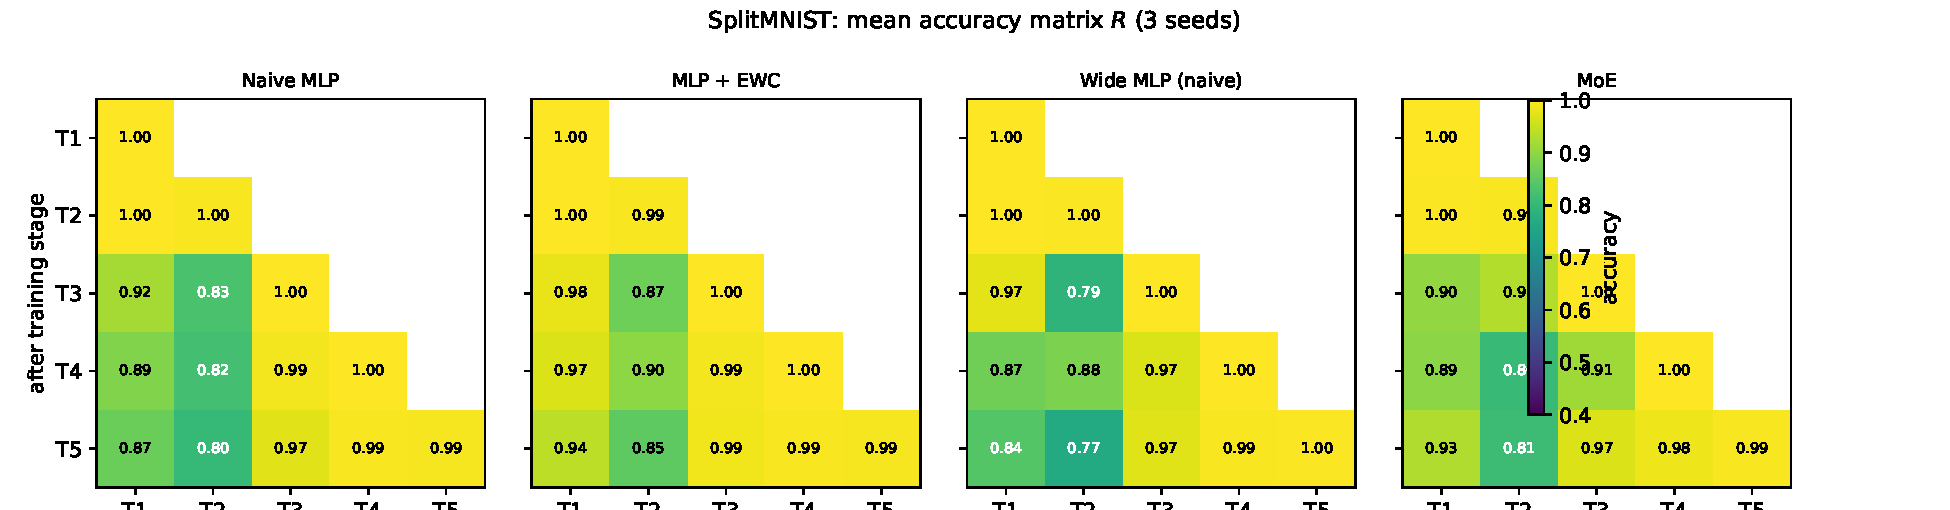
\includegraphics[width=\textwidth]{figures/accmatrix_split_mnist.pdf}
  \caption{Mean accuracy matrix $R$ on SplitMNIST. Entry $(i,j)$ is the
  test accuracy on task $j$ after training task $i$; a column that stays
  bright towards the bottom indicates good retention of that task.}
  \label{fig:accmatrix_split}
\end{figure}

\begin{figure}[H]
  \centering
  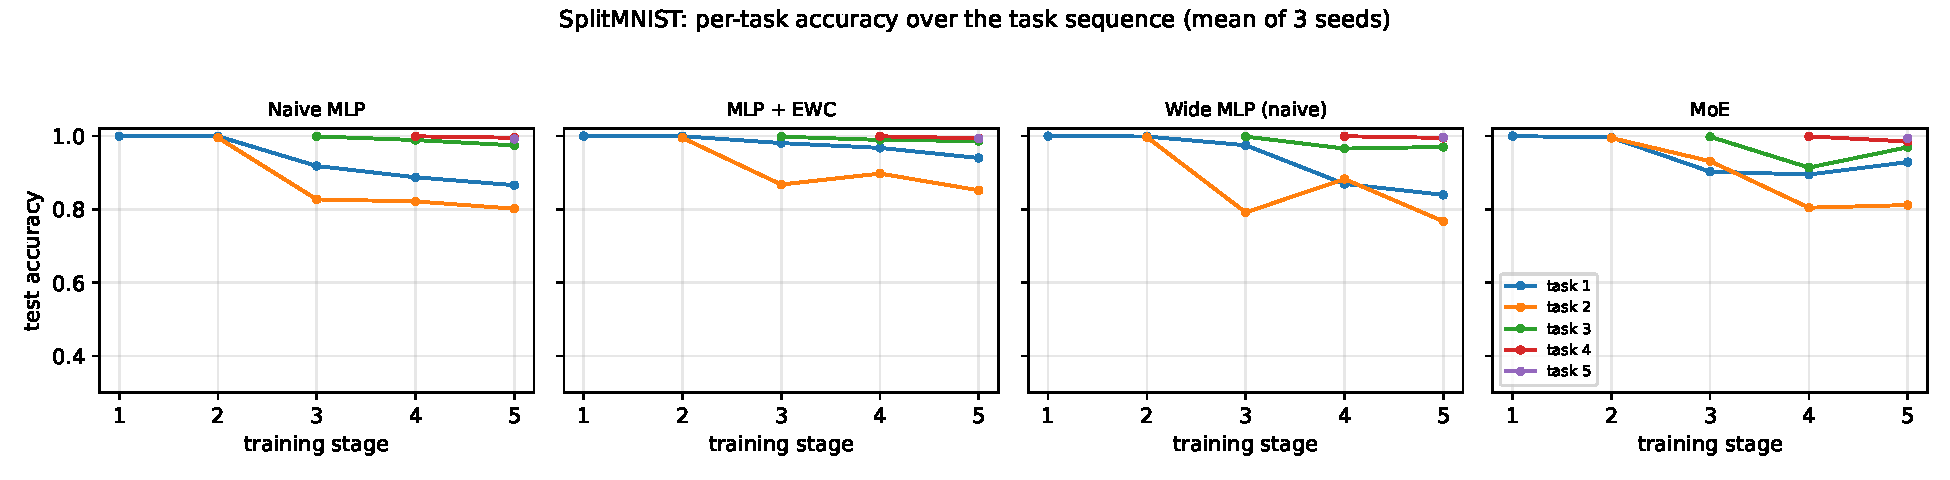
\includegraphics[width=\textwidth]{figures/curves_split_mnist.pdf}
  \caption{Development of the per task test accuracy on SplitMNIST over the
  five training stages (mean of three seeds).}
  \label{fig:curves_split}
\end{figure}

Three observations stand out. First, forgetting is clearly visible in the
unprotected baselines: the naive MLP loses on average $8.9$ percentage
points of previously acquired accuracy, and the wide MLP loses even more
($10.6$ points), although both keep the accuracy of the current task close
to perfect while they train on it. The forgetting is concentrated in the
second task, whose accuracy drops from about $0.99$ to about $0.80$ in the
naive model.

Second, the MoE model reduces the forgetting to $7.4$ points and reaches an
average accuracy of $0.9375$, clearly above the naive baseline ($0.9256$)
and the wide baseline ($0.9135$). Since the wide baseline has about $30$
percent more parameters than the MoE model but performs worst of all, the
advantage of the MoE model cannot be explained by its larger capacity. It
must come from the routed structure itself, which answers the fairness
question SP4 of Section~3.1 for this benchmark.

Third, EWC remains the strongest method on this benchmark ($0.9528$ average
accuracy, $5.5$ points forgetting). The MoE model closes roughly half of
the gap between the naive baseline and EWC without any stored importance
statistics or penalty terms, purely through its architecture.

\section{Results on PermutedMNIST}
\label{sec:resperm}

Table~\ref{tab:results_permuted_mnist} and Figures~7.4 and~7.5 show the corresponding results on
PermutedMNIST, the harder of the two benchmarks.

\begin{table}[H]
  \centering
  \small
  \caption{Results on PermutedMNIST (mean $\pm$ standard deviation over three seeds; best value per column in bold).}
  \label{tab:results_permuted_mnist}
  \begin{tabular}{lccc}
    \toprule
    \textbf{Approach} & \textbf{Avg.\ accuracy} $\uparrow$ & \textbf{Avg.\ forgetting} $\downarrow$ & \textbf{BWT} $\uparrow$ \\
    \midrule
    Naive MLP & $0.8036 \pm 0.0121$ & $0.2179 \pm 0.0144$ & $-0.2179 \pm 0.0144$ \\
    MLP + EWC & \textbf{$0.9318 \pm 0.0141$} & \textbf{$0.0566 \pm 0.0172$} & \textbf{$-0.0566 \pm 0.0172$} \\
    Wide MLP (naive) & $0.9051 \pm 0.0139$ & $0.0933 \pm 0.0182$ & $-0.0933 \pm 0.0182$ \\
    MoE & $0.7307 \pm 0.0365$ & $0.3063 \pm 0.0458$ & $-0.3063 \pm 0.0458$ \\
    \bottomrule
  \end{tabular}
\end{table}


\begin{figure}[H]
  \centering
  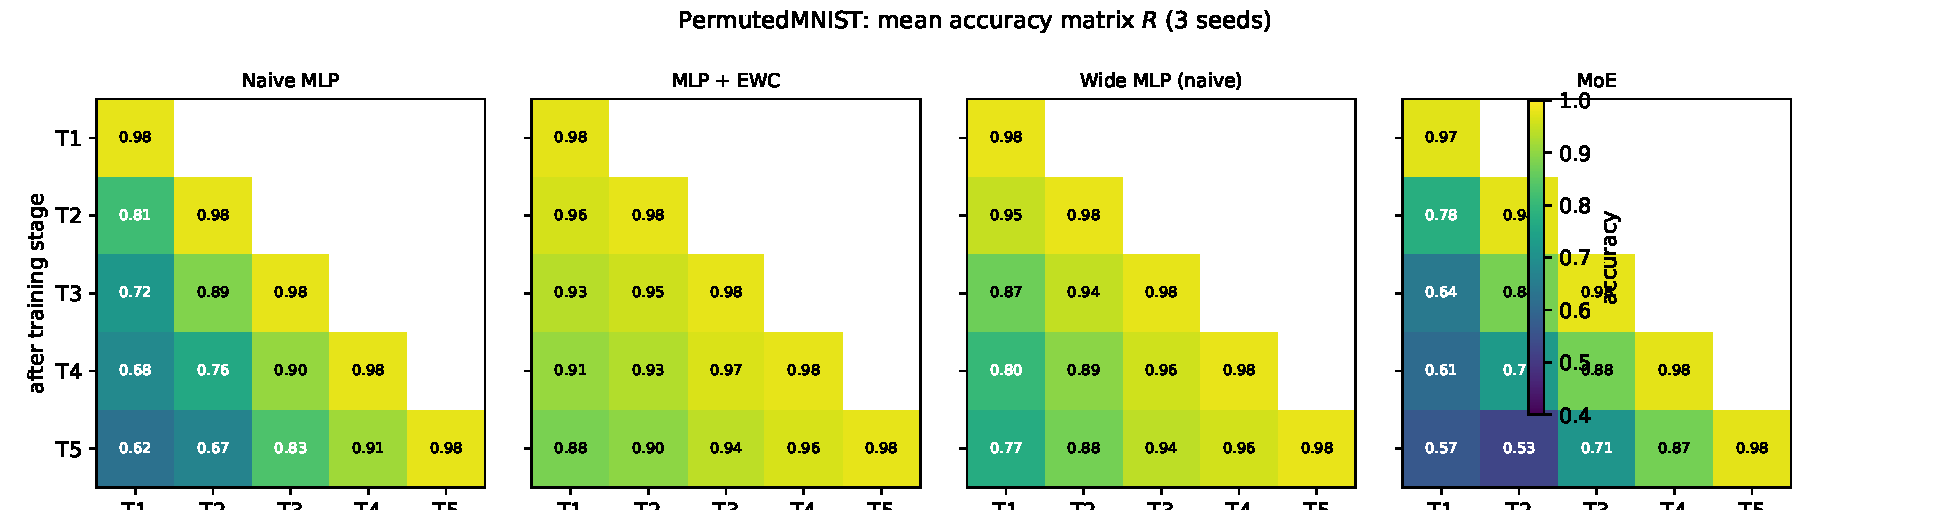
\includegraphics[width=\textwidth]{figures/accmatrix_permuted_mnist.pdf}
  \caption{Mean accuracy matrix $R$ on PermutedMNIST.}
  \label{fig:accmatrix_permuted}
\end{figure}

\begin{figure}[H]
  \centering
  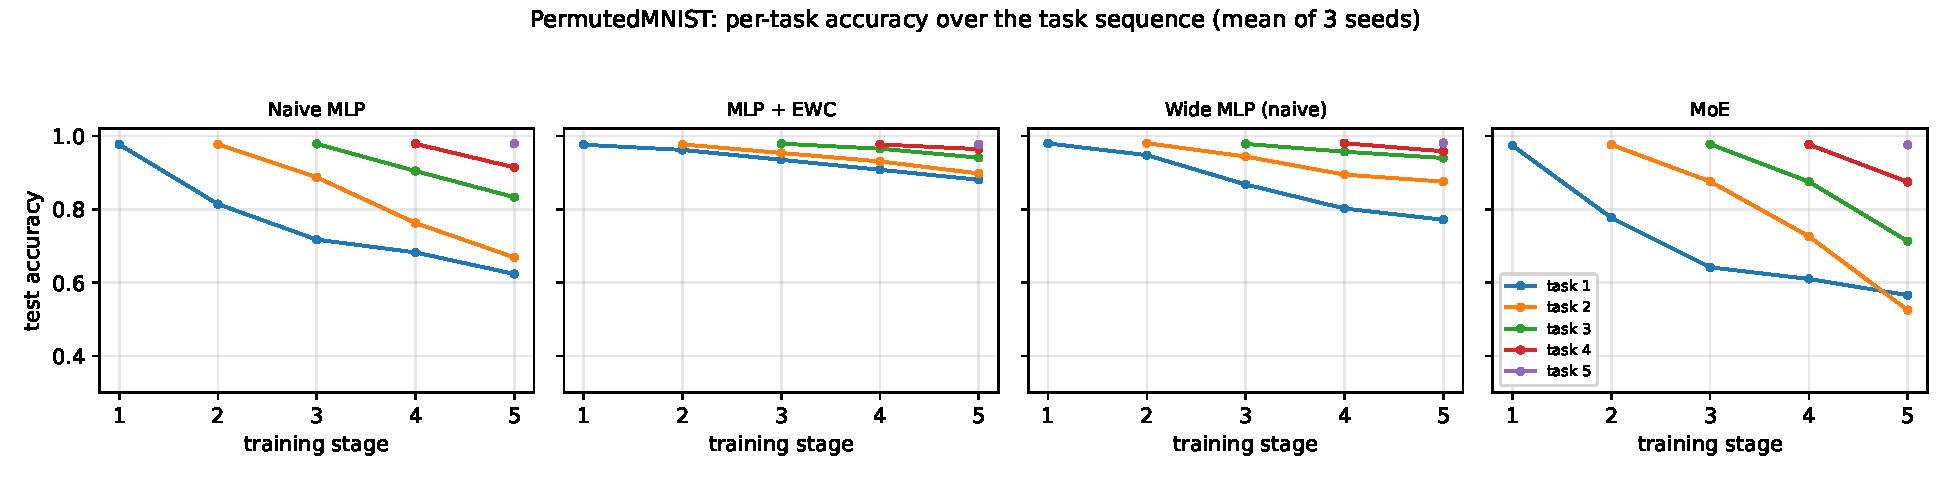
\includegraphics[width=\textwidth]{figures/curves_permuted_mnist.pdf}
  \caption{Development of the per task test accuracy on PermutedMNIST over
  the five training stages (mean of three seeds).}
  \label{fig:curves_permuted}
\end{figure}

On this benchmark, the naive baseline forgets heavily ($21.8$ points,
average accuracy $0.8036$), and EWC again protects effectively ($5.7$
points, average accuracy $0.9318$). Two results, however, were not expected
when the experiments were planned:

\begin{enumerate}[label=\textbf{F\arabic*.}, leftmargin=3em]
  \item The wide baseline beats the naive baseline clearly ($0.9051$
        versus $0.8036$ average accuracy). On a domain incremental
        benchmark, where every task reuses the same classes, simply having
        more than four times the parameters already absorbs a large part of
        the interference. Capacity alone is therefore a strong competitor
        on PermutedMNIST, much stronger than on SplitMNIST, where the wide
        baseline was worst.
  \item The MoE model with the standard load balancing setting performs
        worst of all approaches (average accuracy $0.7307$, forgetting
        $30.6$ points). This contradicted the project hypothesis and
        motivated the analysis in the next section.
\end{enumerate}

\section{Analysis of the PermutedMNIST Failure}
\label{sec:ablation}

The weak PermutedMNIST result of the MoE model was investigated in two
steps. The first suspect was the auxiliary loss for load balancing from
Equation~\eqref{eq:lb}. It pushes the router to use all experts uniformly
within every batch, and because every task is trained separately, this
pressure acts per task: every task is individually encouraged to spread its
samples over all eight experts. But if every task uses every expert, no
expert is task specific, and the very mechanism that should protect old
knowledge is switched off.

To test this explanation, the MoE model was retrained on PermutedMNIST with
a ten times weaker coefficient ($\alpha = 0.001$) and completely without
the auxiliary loss ($\alpha = 0$), again with three seeds. Table~\ref{tab:ablation} shows
the results.

\begin{table}[H]
  \centering
  \small
  \caption{Ablation of the load-balancing coefficient $\alpha$ on PermutedMNIST (mean $\pm$ std over three seeds).}
  \label{tab:ablation}
  \resizebox{\textwidth}{!}{%
  \begin{tabular}{lccc}
    \toprule
    \textbf{MoE variant} & \textbf{Avg.\ accuracy} $\uparrow$ & \textbf{Avg.\ forgetting} $\downarrow$ & \textbf{BWT} $\uparrow$ \\
    \midrule
    MoE ($\alpha = 0.01$, main setting) & $0.7307 \pm 0.0365$ & $0.3063 \pm 0.0458$ & $-0.3063 \pm 0.0458$ \\
    MoE ($\alpha = 0.0$) & $0.7935 \pm 0.0103$ & $0.2293 \pm 0.0127$ & $-0.2293 \pm 0.0127$ \\
    MoE ($\alpha = 0.001$) & $0.7493 \pm 0.0101$ & $0.2851 \pm 0.0129$ & $-0.2851 \pm 0.0129$ \\
    \bottomrule
  \end{tabular}}%
\end{table}


The ablation confirms the load balancing effect, but only partly.
Weakening the coefficient improves the metrics slightly, and removing the
auxiliary loss completely brings the MoE model back to the level of the
naive baseline (average accuracy $0.7935$ versus $0.8036$). The uniform
usage pressure therefore really harms the task specialisation, and the
monotonic improvement across the three coefficients makes this dose
dependent effect clearly visible. However, even without any load balancing
loss, the MoE model does not beat the naive baseline on this benchmark. A
second, deeper cause must exist.

A closer look at the architecture reveals it. In the hidden level design of
Figure~4.2, the router sits behind a shared trunk. On PermutedMNIST, the
difference between two tasks is exactly a different wiring of the input
pixels, that is, the task specific information lives in the input side
mapping, which is stored in the shared trunk in front of the router. Every
new task must rewrite the weights of the trunk, and the router cannot
protect them, because all tasks pass through the same trunk no matter which
experts they use afterwards. On SplitMNIST, by contrast, all tasks share
the same pixel statistics, so one trunk serves all tasks well and routing
behind the trunk is sufficient.

This analysis makes a testable prediction: moving the MoE layer to the
input, so that the input side mapping itself is distributed over experts,
should protect the part of the network where PermutedMNIST tasks actually
differ. The next section tests this prediction.

\section{Architecture Variant with Input Level Routing}
\label{sec:inputlevel}

To test the prediction of Section~7.4, a second MoE architecture was
implemented. In this variant, the router reads the raw input and
distributes eight experts over the $784$ dimensional input space, with an
expert dimension of $256$, followed by a small shared hidden layer and the
usual output heads. The parameter count of $1.68$ million stays comparable
to the hidden level MoE ($1.60$ million) and below the wide baseline
($2.07$ million). Input level routing is also plausible from the router's
point of view: the permutations of PermutedMNIST are linearly well
separable, so a linear gate on raw pixels can learn to tell the tasks
apart, while the same gate behind a shared trunk cannot see the difference
that the trunk has already mixed. The training protocol, the
hyperparameters and the load balancing setting ($\alpha = 0.01$) are
identical to the main experiment; only the position of the MoE layer
changes. Table~\ref{tab:v2} compares the variant with all other approaches on both
benchmarks.

\begin{table}[H]
  \centering
  \small
  \caption{Input-level MoE compared to all approaches on both benchmarks (mean $\pm$ std over three seeds).}
  \label{tab:v2}
  \resizebox{\textwidth}{!}{%
  \begin{tabular}{llccc}
    \toprule
    \textbf{Benchmark} & \textbf{Approach} & \textbf{Avg.\ accuracy} $\uparrow$ & \textbf{Avg.\ forgetting} $\downarrow$ & \textbf{BWT} $\uparrow$ \\
    \midrule
    \multirow{5}{*}{PermutedMNIST} & Naive MLP & $0.8036 \pm 0.0121$ & $0.2179 \pm 0.0144$ & $-0.2179 \pm 0.0144$ \\
    & MLP + EWC & $0.9318 \pm 0.0141$ & $0.0566 \pm 0.0172$ & $-0.0566 \pm 0.0172$ \\
    & Wide MLP (naive) & $0.9051 \pm 0.0139$ & $0.0933 \pm 0.0182$ & $-0.0933 \pm 0.0182$ \\
    & MoE & $0.7307 \pm 0.0365$ & $0.3063 \pm 0.0458$ & $-0.3063 \pm 0.0458$ \\
    & MoE (input-level) & $0.7836 \pm 0.0313$ & $0.2344 \pm 0.0388$ & $-0.2344 \pm 0.0388$ \\
    \midrule
    \multirow{5}{*}{SplitMNIST} & Naive MLP & $0.9256 \pm 0.0295$ & $0.0890 \pm 0.0375$ & $-0.0890 \pm 0.0375$ \\
    & MLP + EWC & $0.9528 \pm 0.0257$ & $0.0551 \pm 0.0320$ & $-0.0551 \pm 0.0320$ \\
    & Wide MLP (naive) & $0.9135 \pm 0.0199$ & $0.1057 \pm 0.0249$ & $-0.1057 \pm 0.0249$ \\
    & MoE & $0.9375 \pm 0.0218$ & $0.0741 \pm 0.0271$ & $-0.0741 \pm 0.0271$ \\
    & MoE (input-level) & $0.9647 \pm 0.0149$ & $0.0391 \pm 0.0183$ & $-0.0391 \pm 0.0183$ \\
    \bottomrule
  \end{tabular}}%
\end{table}


The results confirm the prediction of Section~7.4. On PermutedMNIST, the
input level MoE clearly improves over the hidden level variant: the
average accuracy rises from $0.731$ to $0.784$ and the average forgetting
drops from $0.306$ to $0.234$. This recovery of a large part of the
deficit supports the diagnosis that the shared trunk in front of the
router was the weak point, because routing the raw input protects exactly
the input side mapping that PermutedMNIST overwrites. At the same time
the variant stays slightly below the naive baseline on this benchmark, so
input level routing alone does not fully solve the domain incremental
case; the remaining gap suggests that the shared hidden layer behind the
experts still mixes information from all permutations. On SplitMNIST, the
variant achieves the best result of all compared approaches, with an
average forgetting of only $3.9$ points, better than EWC. The two
variants together show that the position of the router in the
architecture decides whether the MoE idea works in a continual setting:
routing protects only the parameters behind the router, so the router has
to sit where the tasks differ.

\section{Router Analysis}
\label{sec:routeranalysis}

The router profiles, that is, the mean gate probability of every expert on
the test data of every task, make the mechanism behind these results
directly visible. Figure~7.6 shows the profile on SplitMNIST for the
hidden level model, Figure~7.7 shows the profile on PermutedMNIST for the
hidden level model with the main setting, Figure~7.8 shows the profile of
the input level variant on PermutedMNIST, and Figure~7.9 quantifies the
pairwise similarity of the per task routing distributions by their cosine
similarity.

\begin{figure}[H]
  \centering
  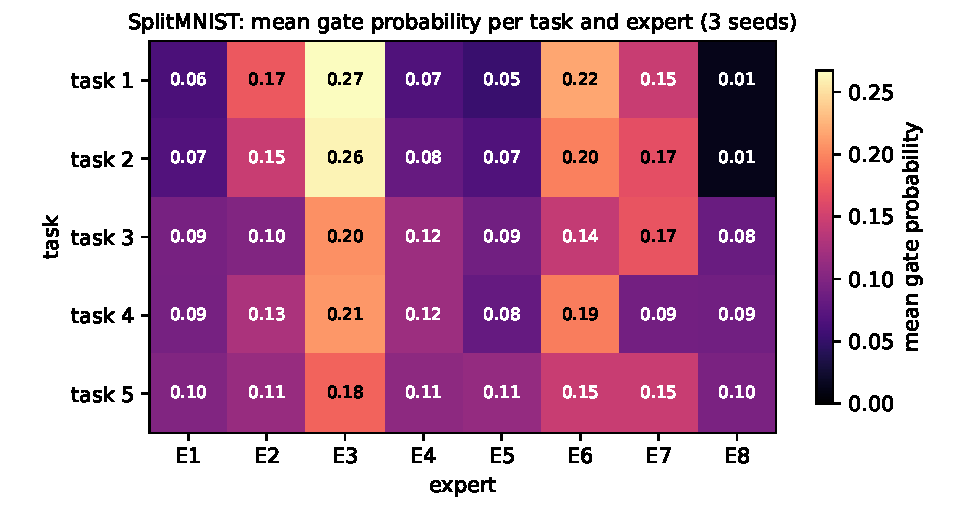
\includegraphics[width=0.8\textwidth]{figures/router_split_mnist.pdf}
  \caption{Router profile of the hidden level MoE on SplitMNIST: mean gate
  probability of every expert for every task (mean over three seeds).}
  \label{fig:router_split}
\end{figure}

\begin{figure}[H]
  \centering
  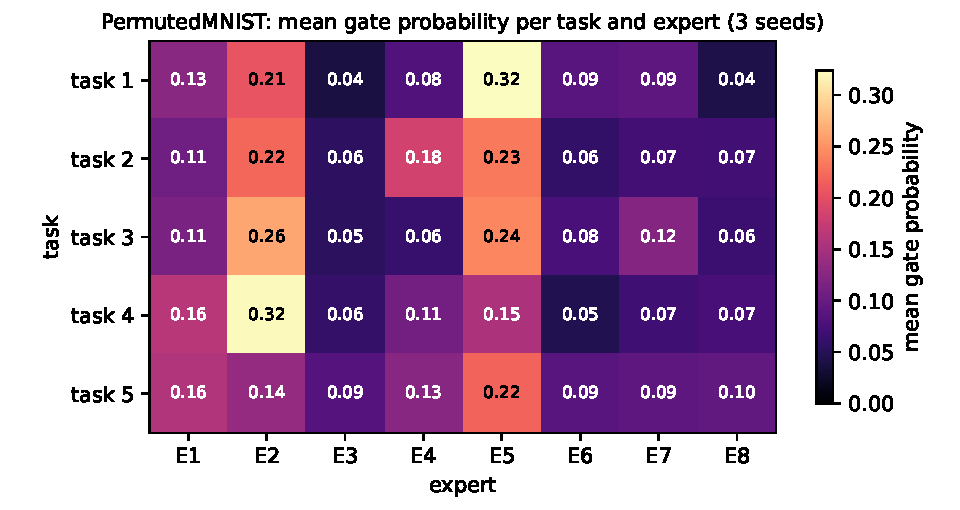
\includegraphics[width=0.8\textwidth]{figures/router_permuted_mnist.pdf}
  \caption{Router profile of the hidden level MoE on PermutedMNIST with the
  main setting. All tasks concentrate on the same two experts E2 and E5,
  which explains the strong forgetting on this benchmark.}
  \label{fig:router_permuted}
\end{figure}

\begin{figure}[H]
  \centering
  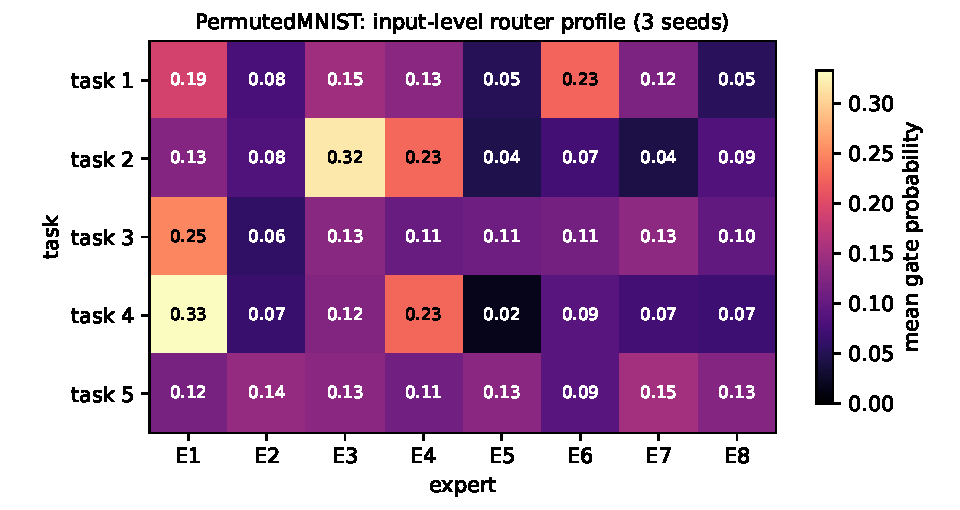
\includegraphics[width=0.8\textwidth]{figures/router_v2_permuted_mnist.pdf}
  \caption{Router profile of the input level MoE on PermutedMNIST. The
  tasks are distributed over clearly different expert subsets.}
  \label{fig:router_v2}
\end{figure}

\begin{figure}[H]
  \centering
  \begin{subfigure}[b]{0.48\textwidth}
    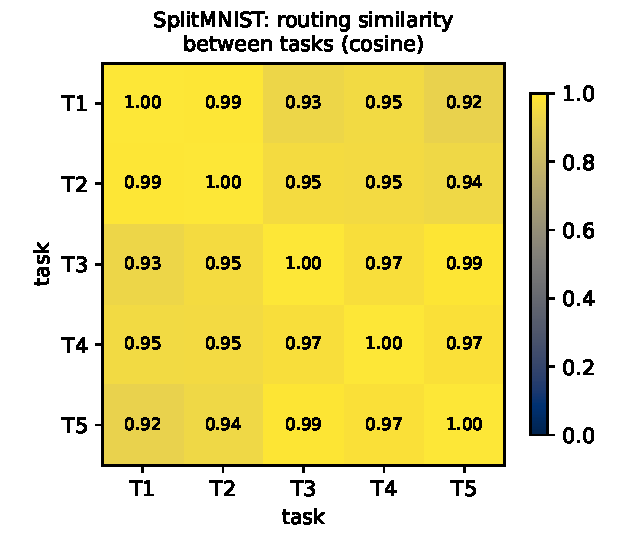
\includegraphics[width=\textwidth]{figures/overlap_split_mnist.pdf}
    \caption{SplitMNIST, hidden level}
  \end{subfigure}
  \hfill
  \begin{subfigure}[b]{0.48\textwidth}
    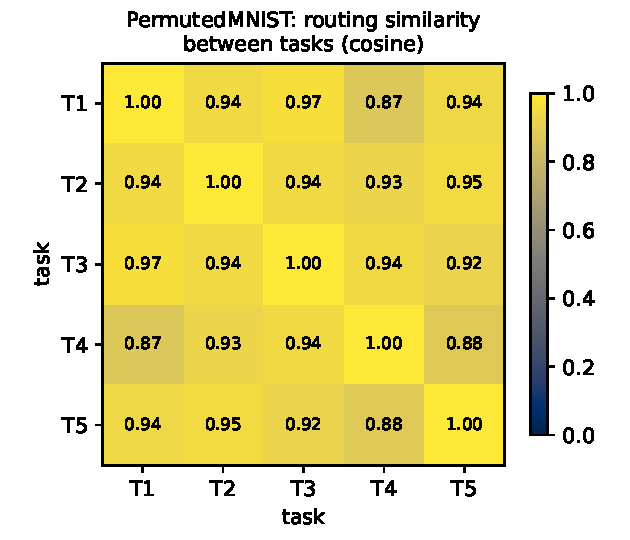
\includegraphics[width=\textwidth]{figures/overlap_permuted_mnist.pdf}
    \caption{PermutedMNIST, hidden level}
  \end{subfigure}
  \caption{Cosine similarity between the per task routing distributions.
  Off diagonal values close to $1$ mean that two tasks use the experts in
  nearly the same way, which indicates a high interference risk; smaller
  values indicate task specific routing.}
  \label{fig:overlap}
\end{figure}

On SplitMNIST, the router develops a differentiated assignment: tasks 1
and 2 prefer the experts E3, E6 and E7, while later tasks distribute their
probability mass more broadly and increasingly use E4 and E8, which were
almost unused at the beginning. The routing is far from a perfectly
disjoint partition, because E3 and E6 are shared by all tasks, which
matches the observation that forgetting is reduced but not eliminated on
this benchmark.

On PermutedMNIST with the hidden level model, the picture is completely
different: every task routes most of its probability mass to the same two
experts E2 and E5, with up to $0.32$ each, and the pairwise routing
similarities in Figure~7.9 are correspondingly close to one. With all
tasks writing to the same experts, the interference is maximal. This is the
direct, measurable cause of the poor result of the main setting on this
benchmark.

The input level variant finally shows the desired behaviour on
PermutedMNIST as well (Figure~7.8): the tasks occupy clearly different
expert subsets, so the gradient updates of a new task mainly rewrite
experts that carry little old knowledge. The router analysis thereby
confirms the central hypothesis of the project at the mechanism level, and
it also explains under which conditions the mechanism can work at all.

\section{Per Task Analysis}
\label{sec:pertask}

The summary metrics compress the behaviour of a run into two numbers.
Table~\ref{tab:pertask} resolves the final accuracy per task and gives a more detailed
picture of where the approaches differ.

\begin{table}[H]
  \centering
  \small
  \caption{Final test accuracy per task after the complete task sequence (mean over three seeds).}
  \label{tab:pertask}
  \begin{tabular}{llccccc}
    \toprule
    \textbf{Benchmark} & \textbf{Approach} & \textbf{T1} & \textbf{T2} & \textbf{T3} & \textbf{T4} & \textbf{T5} \\
    \midrule
    \multirow{4}{*}{SplitMNIST} & Naive MLP & 0.8657 & 0.8015 & 0.9742 & 0.9950 & 0.9918 \\
    & MLP + EWC & 0.9398 & 0.8516 & 0.9861 & 0.9935 & 0.9928 \\
    & Wide MLP (naive) & 0.8392 & 0.7671 & 0.9699 & 0.9946 & 0.9965 \\
    & MoE & 0.9286 & 0.8115 & 0.9692 & 0.9847 & 0.9933 \\
    \midrule
    \multirow{4}{*}{PermutedMNIST} & Naive MLP & 0.6235 & 0.6686 & 0.8329 & 0.9143 & 0.9786 \\
    & MLP + EWC & 0.8803 & 0.8976 & 0.9406 & 0.9639 & 0.9767 \\
    & Wide MLP (naive) & 0.7714 & 0.8754 & 0.9400 & 0.9581 & 0.9807 \\
    & MoE & 0.5655 & 0.5250 & 0.7129 & 0.8746 & 0.9757 \\
    \bottomrule
  \end{tabular}
\end{table}


On SplitMNIST, all approaches keep the three later tasks almost perfectly;
the differences are concentrated in the first two tasks, which were trained
earliest and had the most time to be overwritten. Task~2 is the critical
one: the naive MLP drops to $0.80$, the wide MLP even to $0.77$, while the
MoE model holds $0.81$ and EWC holds $0.85$. The input level variant, which
is not listed separately in the table, reaches the highest retention of
all. A plausible reason for the special role of task~2 is its position in
the sequence: it is early enough to be overwritten by three later tasks,
but its two digit classes are visually more diverse than the classes $0$
and $1$ of the first task, so it is harder to relearn from shared
features.

On PermutedMNIST, the pattern is much more regular. Every approach shows a
monotone gradient: the older a task, the lower its final accuracy. This is
the expected signature of a shared representation that is gradually
overwritten. The gradient is steepest for the hidden level MoE, whose
first task falls to $0.57$, and flattest for EWC, which still reaches
$0.88$ on the first task after the complete sequence. The wide baseline
lies clearly above the naive baseline on the early tasks, which confirms
again that raw capacity helps on this benchmark, while the hidden level MoE
lies below both, which confirms that its failure is structural and not a
capacity problem.

The per task view also shows why the average forgetting of the MoE model
on PermutedMNIST is so large: the model does not lose all tasks equally
but sacrifices exactly the oldest ones, which is consistent with the router
profile in Figure~7.7, where all tasks compete for the same few experts
and the latest task wins.

\section{Discussion}
\label{sec:discussion}

Taken together, the experiments answer the research question of this
project in a differentiated way.

\paragraph{Does MoE reduce forgetting?} Yes, when the routing is allowed to
specialise and when the router sits at the right position in the
architecture. On SplitMNIST, the hidden level MoE clearly outperforms both
the naive and the capacity matched wide baseline. On PermutedMNIST, the
input level MoE recovers a large part of the lost retention and its
router separates the tasks again, although it stays slightly below the
naive baseline in average accuracy. The wide baseline provides the control that isolates the
mechanism: raw capacity helps only where the tasks share the input
distribution, while routing helps where the router can separate the tasks.

\paragraph{What is the role of the router?} The router acts as a learned,
unsupervised task assignment module. Its profiles show that task
specialisation emerges from ordinary training, and they also show the two
conditions under which it fails: a too strong load balancing pressure,
which forces uniform usage per task, and a shared trunk in front of the
router, which mixes the very information that distinguishes the tasks. Both
conditions could be identified only because the router behaviour is
directly inspectable, which is itself an advantage of the MoE approach over
implicit mechanisms.

\paragraph{How does MoE compare to EWC?} EWC is a strong and robust method
on both benchmarks and stays attractive because it does not change the
architecture. The best MoE variant reaches or exceeds the EWC retention
level on SplitMNIST, while on PermutedMNIST EWC remains ahead. The two
approaches are, however, complementary rather than competing: a routed
architecture combined with a light regularisation on the shared components
or on the gate itself is a promising combination for future work.

\paragraph{Threats to validity.} The study is limited to two MNIST based
benchmarks with five tasks each and moderate network sizes; three seeds
give a first estimate of the run to run variability but not a tight
statistical bound. The results should therefore be read as a controlled
proof of concept rather than as evidence for arbitrarily hard continual
learning problems. Within these limits, however, every claim made in this
chapter is backed by a measured and reproducible experiment.
